% !TeX root = ../../tesi.tex

During the internship period and the initial deployment of the project, several practical challenges emerged that required dedicated engineering solutions.

\subsubsection{Robustness to Power Interruptions}

Throughout the design phase, it was observed that power interruptions occurred frequently within the production facility. Such events resulted in unexpected shutdowns of the embedded devices, interrupting the acquisition pipeline and compromising data continuity. Since the data acquisition process was required to operate autonomously for a two-week period without human intervention, this issue represented a critical risk to the success of the experimental campaign.

To mitigate this problem, the entire software architecture was designed to be resilient to power outages. In particular, the acquisition pipeline was encapsulated within a system service configured to automatically restart upon system boot.\cite{systemd_service_2026}

A \emph{system service} is a background process managed by the operating system's service manager (e.g., \texttt{systemd} in Linux-based systems). Services are designed to:

\begin{itemize}
    \item Automatically start at system boot,
    \item Restart upon unexpected failure,
    \item Run independently of user login sessions,
    \item Provide logging and monitoring capabilities.
\end{itemize}

At both sites, a user-level \texttt{systemd} service was implemented to execute the image acquisition script at startup. The service invokes a dedicated bash launcher script responsible for:

\begin{itemize}
    \item Navigating to the project directory,
    \item Activating the Python virtual environment,
    \item Launching the acquisition or processing script.
\end{itemize}

The service was configured with automatic restart policies (e.g., \texttt{Restart=always}) and a short restart delay to ensure that, upon restoration of electrical power, the system autonomously resumed operation without manual intervention.

This design choice significantly increased the reliability of the deployment and reduced maintenance overhead in the industrial environment.
%% TODO: qui potrei mettere un link al codice per il service

\subsubsection{Illumination Variability at Site 2}

An additional challenge was related to the physical configuration of Site 2. The bread extraction station is located on a metallic and reflective table positioned in front of two large windows (as shown in Figure~\ref{fig:site2}).

This configuration introduced significant illumination variability throughout the day due to:

\begin{itemize}
    \item Natural light intensity fluctuations,
    \item Direct sunlight reflections on the metallic surface,
    \item Shadows generated by operators during manual extraction.
\end{itemize}

Since the primary objective at Site 2 is visual quality assessment of baked bread through an anomaly detection model, uncontrolled illumination variations could directly affect the reliability of model predictions. In particular, variations in brightness and color temperature may introduce systematic biases in RGB-based inference.\cite{hoang_image-based_2025,kuhlechner_object_2025}

To ensure consistency and minimize illumination-related variability, a high-intensity artificial lighting source was installed above the acquisition area (as shown in Figure \ref{fig:faretto_sito2}).
\newline
The artificial illumination:

\begin{itemize}
    \item Increases dominance over ambient light,
    \item Reduces the impact of daylight fluctuations,
    \item Improves the repeatability and stability of color measurements.
\end{itemize}

By stabilizing the lighting conditions, the system achieves more reliable visual inference, which is critical for robust anomaly detection and for detecting deviations in the baking process.\cite{hoang_image-based_2025,kuhlechner_object_2025}

\begin{figure}[h]
    \centering
    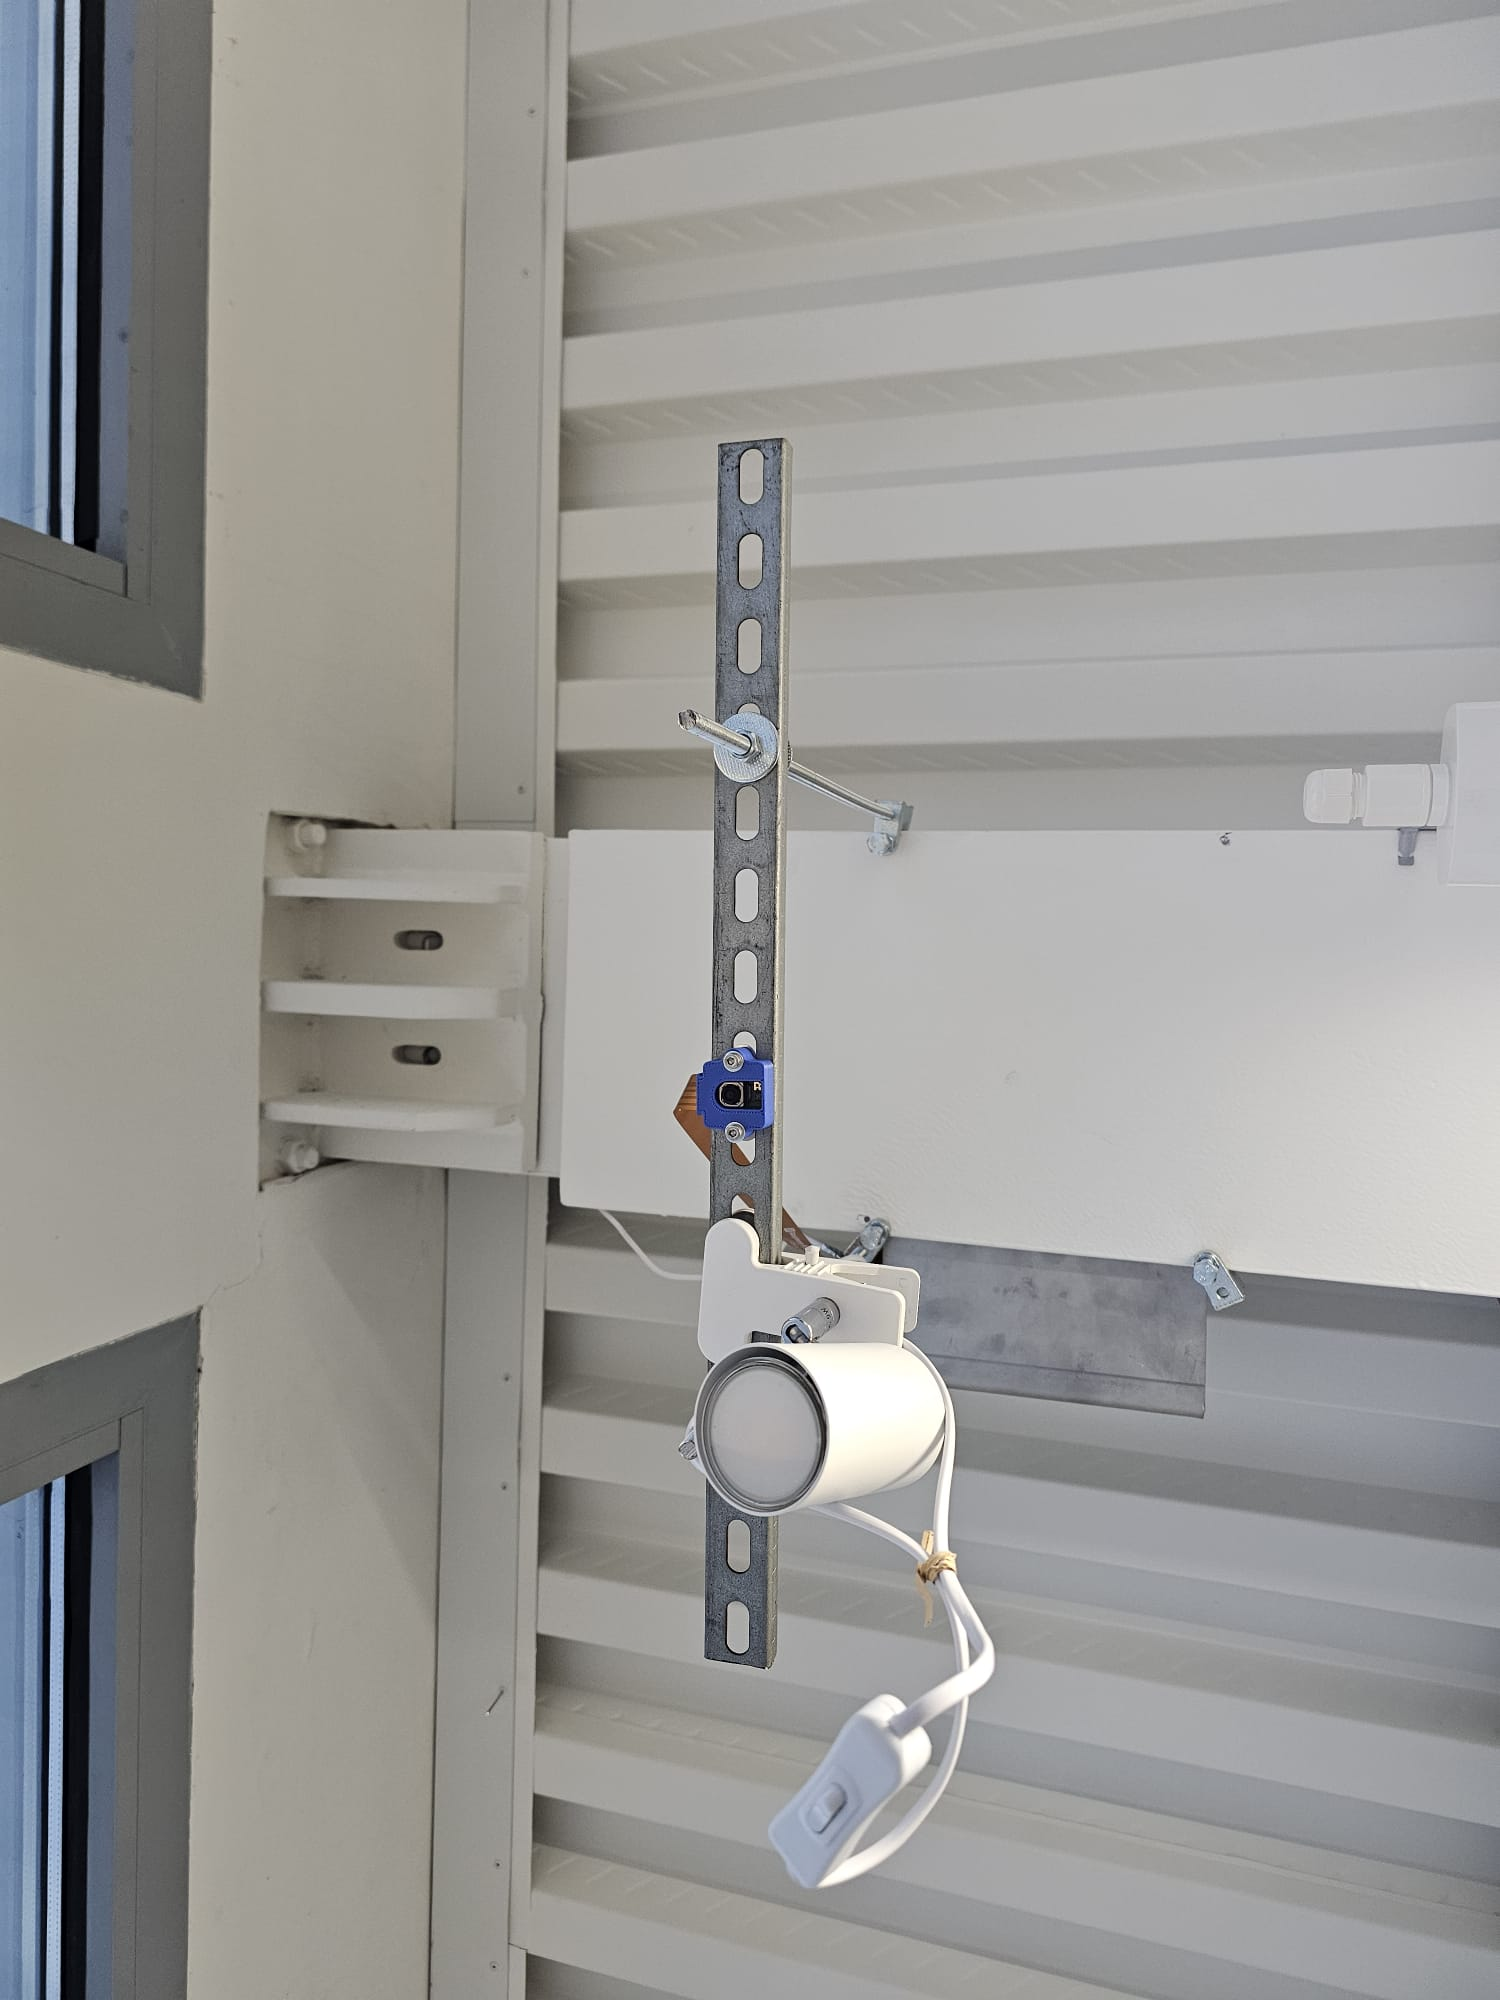
\includegraphics[width=0.5\linewidth, angle=90]{images/faretto_sito_2(1).jpeg}
    \caption{Light source placed next to the Raspberry Pi Camera to illuminate the scene and keep lighting as constant as possible}
    \label{fig:faretto_sito2}
\end{figure}
